\section{Pendahuluan}
\subsection{Latar Belakang}
IPv4 (Internet Protocol versi 4) adalah protokol yang tidak terpisahkan di 
Internet yang menangani perangkat dan perutean paket melalui jaringan. 
Setiap perangkat dalam jaringan berbasis IPv4 memiliki alamat IP 32-bit, 
yang memungkinkan komunikasi ujung ke ujung di antara host di jaringan lain.

Namun, karena jaringan dipecah menjadi subnet dan internet terdiri jaringan 
yang saling berhubungan yang tak terhitung jumlahnya, perangkat tidak dapat 
selalu secara langsung berkomunikasi satu sama lain. Sebaliknya, informasi 
harus dirutekan - diteruskan dari jaringan ke jaringan - sampai akhirnya 
mencapai tujuannya.

Perutean adalah proses memilih jalur dalam jaringan yang akan dilalui 
mengirim paket data. Pada IPv4, router melakukan hal ini dengan merutekan 
paket berdasarkan berdasarkan alamat IP tujuan melalui tabel dan algoritma 
perutean.

Crimping adalah teknik mekanis yang digunakan untuk menyambung dua bahan - 
biasanya kabel dan konektor - dengan mengubah bentuk salah satu atau kedua 
komponen untuk membentuk sambungan yang aman tanpa perlu disolder. Teknik 
ini banyak digunakan dalam sistem kelistrikan dan jaringan untuk menciptakan 
pemutusan yang andal, cepat, dan dapat diulang, terutama di lingkungan di 
mana kecepatan dan skalabilitas sangat penting (misalnya, telekomunikasi, 
otomotif, ruang angkasa, dan pemasangan kabel terstruktur).

Proses ini menggunakan alat khusus, yang disebut alat crimping, untuk 
memampatkan terminal logam di sekitar kabel yang dilucuti, menciptakan 
ikatan listrik dan mekanik yang kuat.
\subsection{Dasar Teori}
\begin{enumerate}
	\item Topologi Network

	Jaringan dimodelkan sebagai grafik di mana perangkat (router) adalah 
	simpul dan koneksi (link) adalah sisi. Oleh karena itu, perutean menjadi 
	proses menentukan jalur yang paling efisien melalui grafik ini untuk 
	mengirimkan paket dari sumber ke tujuan. Hal ini dicapai dengan 
	menggunakan tabel perutean, yang dikelola oleh setiap router untuk 
	menentukan ke mana harus meneruskan paket yang masuk. Router 
	membandingkan alamat IP tujuan dalam setiap paket dengan entri dalam 
	tabel perutean, menggunakan kecocokan awalan terpanjang untuk memilih 
	jalur terbaik.

	\item Algoritma Routing

	Perutean dapat berupa statis atau dinamis. Perutean statis bergantung 
	pada jalur yang dikonfigurasi secara manual yang tetap konstan kecuali 
	diperbarui secara manual, sehingga cocok untuk jaringan kecil atau 
	sederhana. Sebaliknya, perutean dinamis beradaptasi dengan perubahan 
	topologi jaringan melalui algoritme khusus. Protokol routing dinamis 
	ini termasuk RIP (Routing Information Protocol), yang menggunakan 
	pendekatan vektor jarak berdasarkan algoritma Bellman-Ford, dan OSPF 
	(Open Shortest Path First), yang menggunakan pendekatan link-state dan 
	algoritma Dijkstra untuk menghitung jalur terpendek. BGP (Border Gateway 
	Protocol), yang biasa digunakan di antara jaringan besar, menggunakan 
	mekanisme vektor jalur dan kebijakan daripada metrik jalur terpendek 
	yang sederhana.

	\item Subnetting
	
	Perutean IPv4 dibentuk oleh penggunaan subnetting dan CIDR (Classless 
	Inter-Domain Routing), yang memungkinkan alokasi alamat IP yang lebih 
	fleksibel dengan mendefinisikan ukuran jaringan dengan awalan (contoh, 
	/24).

	\item Crimping
	
	Crimping didukung oleh konsep teoretis dari ilmu material, deformasi 
	mekanik, dan teknik listrik. Proses ini melibatkan perubahan bentuk 
	terminal logam secara plastis di sekitar kawat menggunakan alat crimping, 
	yang berarti menerapkan kekuatan yang cukup untuk membentuk kembali 
	logam secara permanen tanpa menyebabkan kerusakan. Hal ini dilakukan 
	dengan mengompresi logam melebihi batas elastisitasnya, menghasilkan 
	ikatan permanen yang erat yang sesuai dengan bentuk untaian kawat. 
	Deformasi plastik ini memastikan bahwa konektor dan kawat mencapai 
	kontak yang erat, sering kali menghilangkan oksida permukaan dan 
	kontaminan dalam prosesnya.
\end{enumerate}
%===========================================================%
\section{Tugas Pendahuluan}
Bagian ini berisi jawaban dari tugas pendahuluan yang telah anda kerjakan, beserta penjelasan dari jawaban tersebut
\begin{enumerate}
	\item Karena ada empat departemen yang berbeda, maka kita perlu 
	menggunakan empat subnet yang berbeda untuk masing-masing 
	departemen. Besar subnet yang dibutuhkan dapat dihitung 
	dengan menambah dua pada banyak perangkat dan membulatkan 
	ke atas ke pangkat 2 terdekat.
	{\small
		\begin{center}
		\begin{tabular}{ |c|c|c|c|c|c|c| } 
			\hline
			Departemen & Perangkat & Host yang dibutuhkan & Besar subnet & CIDR & Banyak host & Subnet Address \\
			\hline
			RnD & 100 & $ \geq $ 102 & /25 & /25 & 126 & 192.168.0.0/25 \\
			Produksi & 50 & $ \geq $ 52 & /26 & /26 & 62 & 192.168.0.128/26 \\
			Administrasi & 20 & $ \geq $ 22 & /27 & /27 & 30 & 192.168.0.192/27 \\
			Keuangan & 10 & $ \geq $ 12 & /28 & /28 & 14 & 192.168.0.0/28 \\
			\hline
		\end{tabular}
		\end{center}
	}
	Dapat dilihat bahwa CIDR yang digunakan adalah /25, /26, /27, dan /28.
	Banyak host yang dapat digunakan pada masing-masing subnet adalah 126, 
	62, 30, dan 14. Hal ini karena dua host telah digunakan untuk network 
	address (host pertama) dan broadcast address (host terakhir).
	\item Berikut adalah diagram topologi jaringan yang digunakan 
	pada soal ini. Bila mengabaikan switch pada tiap departemen, 
	maka topologi jaringan ini adalah topologi star. Bila switch 
	dihitung, maka topologi jaringan ini adalah topologi tree.
	\begin{center}
		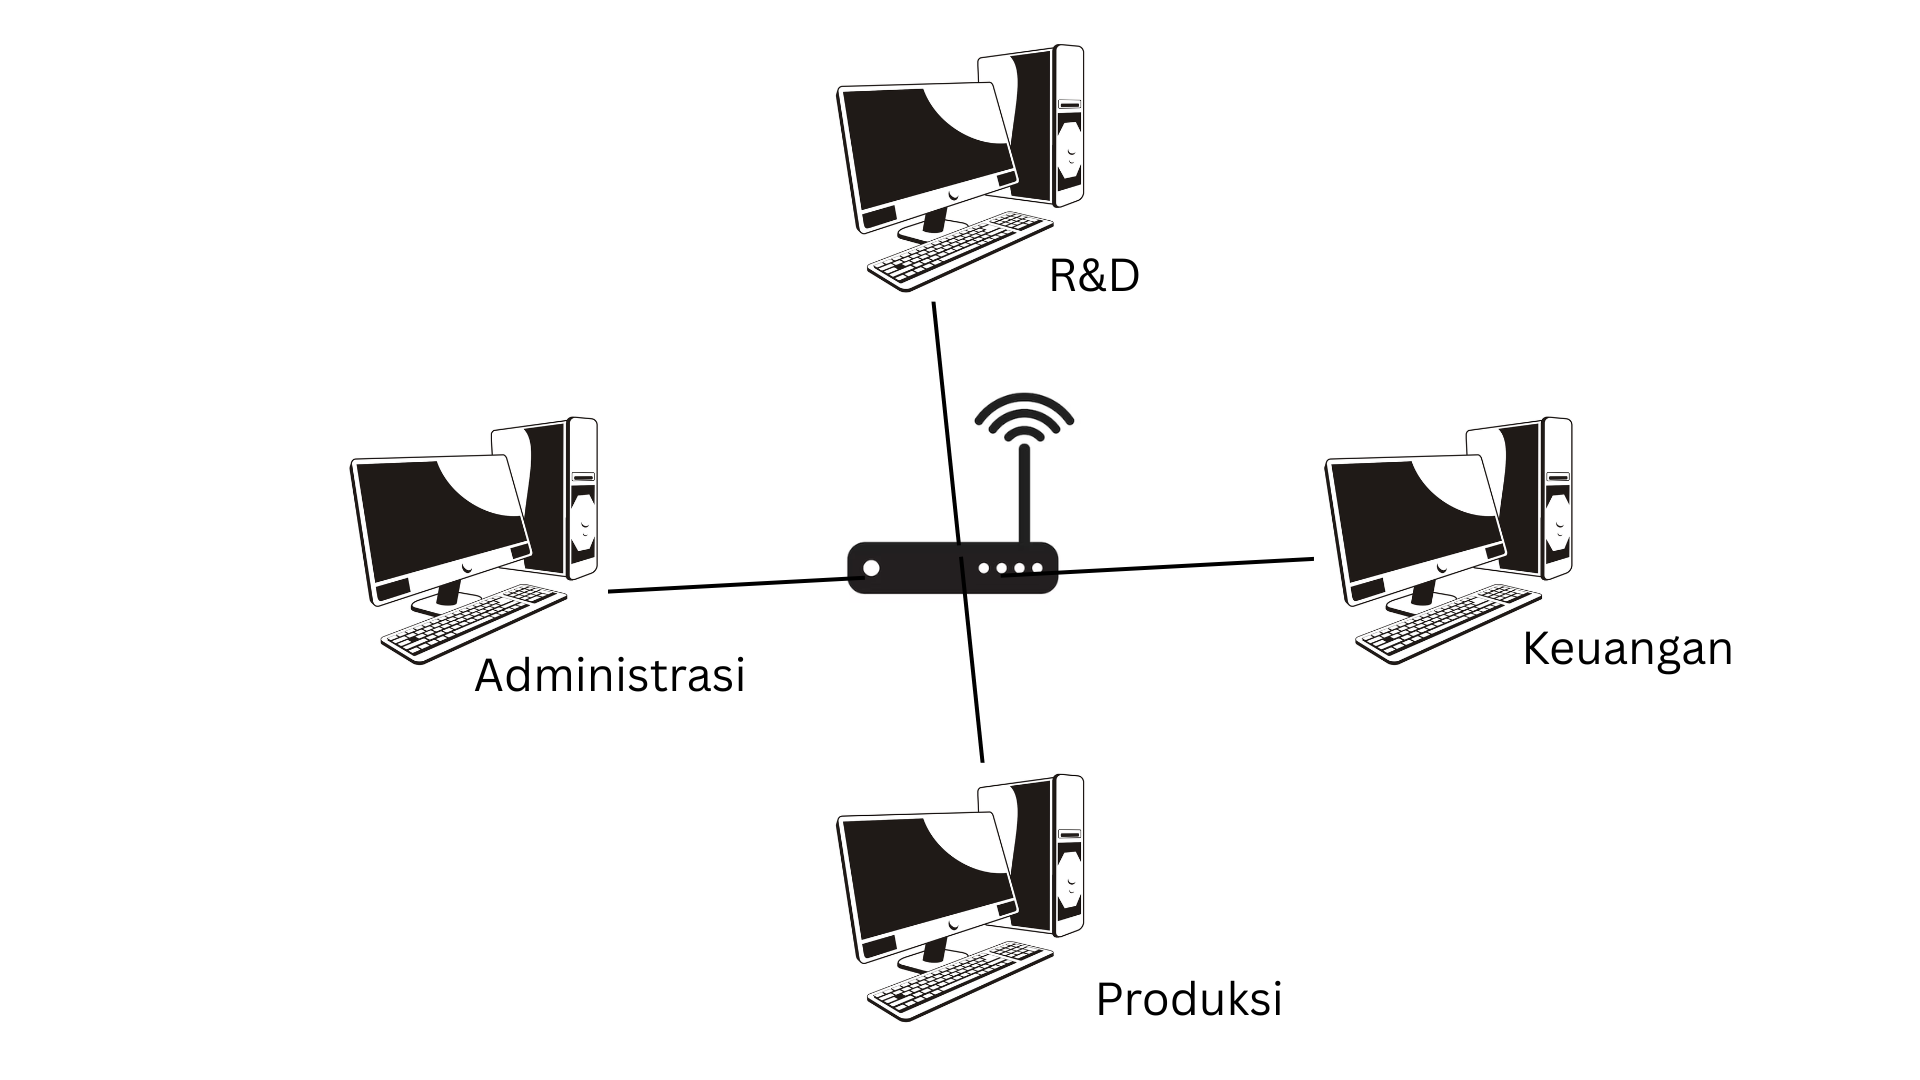
\includegraphics[scale=0.5]{P1/img/topology.png}
    \end{center}
	\item Berikut tabel routing sederhana. Gateway yang digunakan merupakan
	IP pertama dari masing-masing subnet. Hal ini merupakan standar umum 
	pada banyak jaringan, serta dapat mencegah conflict dengan host yang 
	diberi secara dinamis.
	{\small
		\begin{center}
		\begin{tabular}{ |c|c|c|c| } 
			\hline
			Destinasi Network & Netmask/prefix & Default gateway & Interface \\
			\hline
			192.168.0.0 & /25 & 192.168.0.1 & RnD (eth0)  \\
			192.168.0.128 & /26 & 192.168.0.129 & Produksi (eth1)  \\
			192.168.0.192 & /27 & 192.168.0.193 & Administrasi (eth2)  \\
			192.168.0.224 & /28 & 192.168.0.225 & Keuangan (eth3)  \\
			\hline
		\end{tabular}
		\end{center}
	}
	\item Jenis routing yang paling cocok digunakan untuk network 
	ini adalah CIDR dengan static routing. Hal ini karena CIDR 
	digunakan untuk membuat subnet yang efisien, sedangkan 
	static routing digunakan untuk memindahkan paket-paket antara 
	subnet tersebut.

	Dalam network pada soal ini, CIDR berguna untuk memberi IP 
	address menggunakan subnet mask yang flexibel. CIDR dapat 
	memberi IP address yang sesuai dengan kebutuhan dan  
	banyaknya host yang dibutuhkan. Sedangkan static routing 
	digunakan untuk memindahkan paket-paket antar subnet yang 
	telah dibuat oleh CIDR. Karena network pada soal hanya 
	memiliki empat subnet di mana semuanya menuju satu router, 
	maka static routing lebih efisien digunakan dibandingkan
	dynamic routing.
\end{enumerate}